%%%%%%%%%%%%%%%%

% designed to be integrated with conceptual figure

%%%%%%%%%%%
\documentclass[border=0.2cm,11pt]{standalone}
\usepackage{tgheros}
\renewcommand*\familydefault{\sfdefault}%

\usepackage{tikz}
\usetikzlibrary{positioning,automata}
\usetikzlibrary{shapes}

\tikzset{>=latex} % for LaTeX arrow head
\usepackage{xcolor}
\usepackage{ifthen}

% taken from neural networks
\usepackage{amsmath} % for aligned
%\usepackage{amssymb} % for \mathbb
%\usepackage{etoolbox} % for \ifthen
\usepackage{listofitems} % for \readlist to create arrays
\usetikzlibrary{arrows.meta} % for arrow size
\usepackage[outline]{contour} % glow around text
\contourlength{1.4pt}

% using tableau 10 color palette: https://public.tableau.com/views/TableauColors/ColorPaletteswithRGBValues?%3Aembed=y&%3AshowVizHome=no&%3Adisplay_count=y&%3Adisplay_static_image=y

\definecolor{myblue}{RGB}{31,119,180}
\definecolor{myred}{RGB}{214,39,40}
\definecolor{mygreen}{RGB}{44,160,44}

% original colors defined by original author
\colorlet{myorange}{orange!70!red!60!black}
\colorlet{mydarkred}{red!30!black}
\colorlet{mydarkblue}{blue!40!black}
\colorlet{mydarkgreen}{green!30!black}
\tikzstyle{mynode}=[align=center, rounded corners, minimum height=1cm]
\tikzstyle{procs_ecolo}=[mynode, rectangle, fill=mygreen!30]
\tikzstyle{procs_evol}=[mynode, rectangle, fill=myred!30]
\tikzstyle{mechanisms}=[mynode, rectangle, thick, minimum width=3cm]
\tikzstyle{patterns}=[mynode, circle, thick, fill=myblue!20]


% \tikzstyle{node}=[ultra thick,circle,minimum size=30,inner sep=2.,outer sep=0.6]
% \tikzstyle{node green}=[node,fill=mygreen]
% \tikzstyle{node blue}=[node,fill=myblue]
% \tikzstyle{node orange}=[node,orange!20!black,draw=myorange!30!black,fill=myorange!20]
% \tikzstyle{node red}=[node,fill=myred]
\tikzstyle{connect}=[thick,mydarkblue] %,line cap=round
\tikzstyle{connect arrow}=[-{Latex[length=6,width=6]},thick,mydarkblue,shorten <=0.5,shorten >=1]
 

% spacing nodes
% \tikzset{node distance = 0.5cm and 0.5cm}

\begin{document}

 
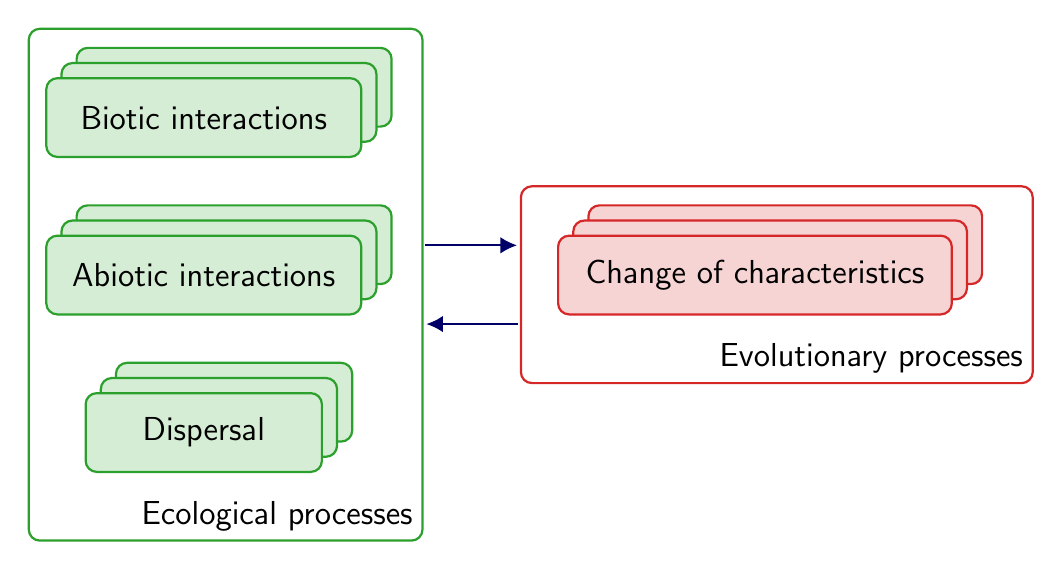
\begin{tikzpicture}[
    node distance=1.5cm,
    on grid,
    very thick,
    font=\large]
 
\node[mechanisms, draw=mygreen, minimum height = 6.5cm, minimum width = 5cm] (model_contour) at (-2.3,-2.7) {};
\node[above left] at (model_contour.south east) {Ecological processes};
\node[mechanisms, draw=myred, minimum height = 2.5cm, minimum width =6.5cm, right=7cm of model_contour] (model_contour2) {};
\node[above left] at (model_contour2.south east) {Evolutionary processes};

\foreach \Z in {1,...,3}{
    \node[mechanisms, fill=mygreen!20,draw=mygreen,minimum width=4cm] at (-2,0,\Z/2) (binter) {\ifthenelse{\Z=3}{Biotic interactions}{}};
    \node[mechanisms, fill=mygreen!20,draw=mygreen,minimum width=4cm] at (-2,-2,\Z/2) (ainter) {\ifthenelse{\Z=3}{Abiotic interactions}{}};
    \node[mechanisms, fill=mygreen!20,draw=mygreen] at (-2,-4,\Z/2) (disp) {Dispersal};
    \node[mechanisms, fill=myred!20,draw=myred,minimum width=5cm] at (5,-2,\Z/2) (char) {\ifthenelse{\Z=3}{Change of characteristics}{}};
};





\begin{scope} [connect arrow]  % now dashed is for the lines inside the scope
    \draw ([yshift=0.5cm]model_contour.east) to ([yshift=0.5cm]model_contour2.west);
    \draw ([yshift=-0.5cm]model_contour2.west) to ([yshift=-0.5cm]model_contour.east);

\end{scope}

\end{tikzpicture}
 
\end{document}